\documentclass[a4paper, 12pt]{article}

%%% SST LAB PROTOCOLL PREAMBLE
%%% 2019
%%%%%%%%%%%%%%%%%%%%%%%%%%%%%%%


%%% PACKAGES
%%%%%%%%%%%%%%%%%%%%%%%%%%%

\usepackage[ngerman]{babel}

\usepackage[utf8]{inputenc}
\usepackage{amsmath}
\usepackage{pgfplots}
\usepackage{tikz}
\usepackage[many]{tcolorbox}
\usepackage{graphicx}
\graphicspath{ {./graphics/} }
\usepackage{pdfpages}
\usepackage{dashrule}
\usepackage{float}
\usepackage{siunitx}
\usepackage{booktabs}
\usepackage[version=4]{mhchem}

%%% DOCUMENT GEOMETRY
%%%%%%%%%%%%%%%%%%%%%%%%%%%

\usepackage{geometry}
\geometry{
 a4paper,
 total={0.6180339887498948\paperwidth,0.6180339887498948\paperheight},
 top = 0.1458980337503154\paperheight,
 bottom = 0.1458980337503154\paperheight
 }
\setlength{\jot}{0.013155617496424828\paperheight}
\linespread{1.1458980337503154}

\setlength{\parskip}{0.013155617496424828\paperheight} % paragraph spacing


%%% COLORS
%%%%%%%%%%%%%%%%%%%%%%%%%%%

\definecolor{red1}{HTML}{f38181}
\definecolor{yellow1}{HTML}{fce38a}
\definecolor{green1}{HTML}{95e1d3}
\definecolor{blue1}{HTML}{66bfbf}
\definecolor{hsblue}{HTML}{00b1db}
\definecolor{hsgrey}{HTML}{afafaf}

%%% CONSTANTS
%%%%%%%%%%%%%%%%%%%%%%%%%%%
\newlength{\smallvert}
\setlength{\smallvert}{0.0131556\paperheight}


%%% COMMANDS
%%%%%%%%%%%%%%%%%%%%%%%%%%%

% differential d
\newcommand*\dif{\mathop{}\!\mathrm{d}}

% horizontal line
\newcommand{\holine}[1]{
  	\begin{center}
	  	\noindent{\color{hsgrey}\hdashrule[0ex]{#1}{1pt}{3mm}}\\%[0.0131556\paperheight]
  	\end{center}
}

% mini section
\newcommand{\minisec}[1]{ \noindent\underline{\textit {#1} } \\}

% quick function plot
\newcommand{\plotfun}[3]{
  \vspace{0.021286\paperheight}
  \begin{center}
    \begin{tikzpicture}
      \begin{axis}[
        axis x line=center,
        axis y line=center,
        ]
        \addplot[draw=red1][domain=#2:#3]{#1};
      \end{axis}
    \end{tikzpicture}
  \end{center}
}

% box for notes
\newcommand{\notebox}[1]{

\tcbset{colback=white,colframe=red1!100!black,title=Note!,width=0.618\paperwidth,arc=0pt}

 \begin{center}
  \begin{tcolorbox}[]
   #1 
  \end{tcolorbox}
 
 \end{center} 
 
}

% box for equation
\newcommand{\eqbox}[2]{
	
	\tcbset{colback=white,colframe=hsblue!100!black,title=,width=#2,arc=0pt}
	
	\begin{center}
		\begin{tcolorbox}[ams align*]
				#1
		\end{tcolorbox}
		
	\end{center} 
	
}

% END OF PREAMBLE

\setlength\columnsep{0.145898\paperwidth}
%%%%%%%%%%%%%%%%%%%%%%%%%%%%%%%%%%%%%

\begin{document}

% 1
%%%%%%%%%%%%%%%%%%%%%%%%%%%%%%%%%%%%%
  
\includepdf{./titlepage/titlepage1.pdf}
  \clearpage
  \setcounter{page}{1}
%%%%%%%%%%%%%%%%%%%%%%%%%%%%%%%%%%%%%

\section{Vorbereitungsaufgaben}

\subsection{Aufbau und Wirkungsweise des BPT}

\begin{center}
  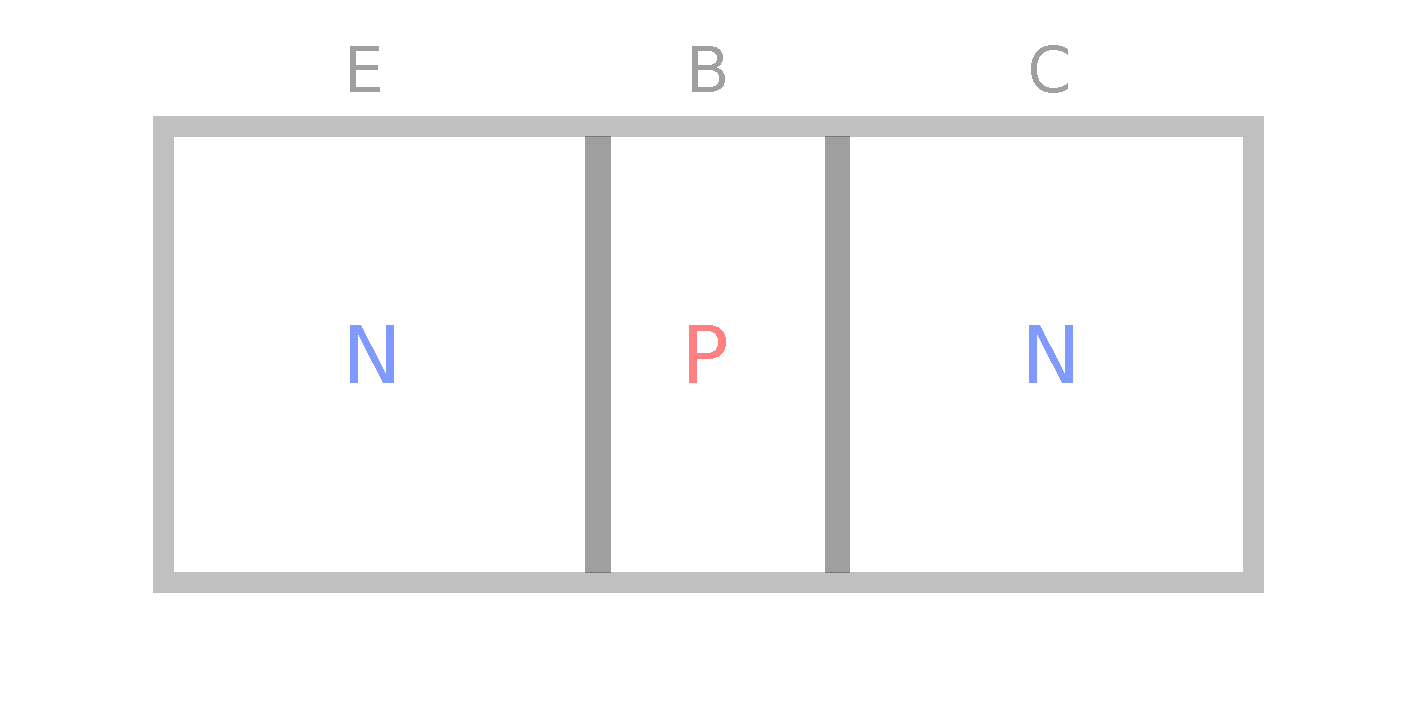
\includegraphics[width=\textwidth]{1_1/npn}
\end{center}

Bipolartransistoren können durch Verkettung von insgesamt 3
dotierten Halbleiterkristallen (vgl. Diode), jeweils entweder p- oder
n-leitend, realisiert werden, woraus sich die beiden Kombinationsarten
\textit{npn} und \textit{pnp} ergeben.

\noindent Die 3 Regionen bezeichnet man als
\begin{itemize}
\item Emitter (E)
\item Basis (B)
\item Kollektor (C)
\end{itemize}

welche in der
Regel unterschiedliche Dotierungskonzentrationen aufweisen. So ist der Emitter
höher als die Basis und die Basis höher als der Kollektor dotiert.


\begin{center}
  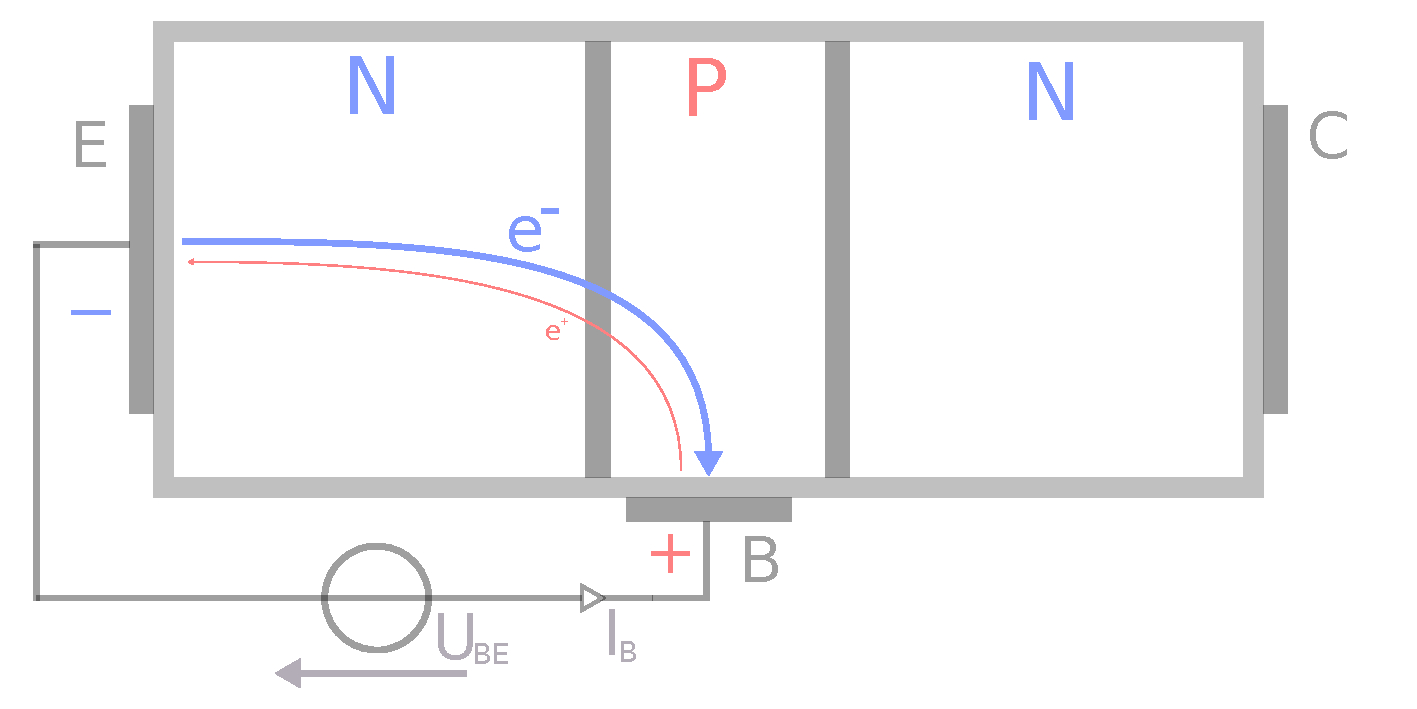
\includegraphics[width=\textwidth]{1_1/npn_voltage}
\end{center}

Legt man von außen eine Spannung $U_\textrm{BE}$ an den Basis-Emitter-Übergang
des Transistors, sodass er in Durchlassrichtung geschaltet
ist\footnote{$U_{\textrm{BE}}>U_\textrm{D}$, $U_\textrm{D}:$ Diffusionsspannung
  ($0.7 \,\ \si{\volt}$)}, so wird dieser leitend und lässt einen (kleinen) Basisstrom
$I_B$ fließen. Da der Emitter deutlich höher dotiert ist als die Basis,
überwiegt beim Basisstrom der Majoritätsträgerstrom der Elektronen vom Emitter in
die Basis (gegenüber
dem Strom der Defektelektronen von der Basis in den Emitter).

\begin{center}
  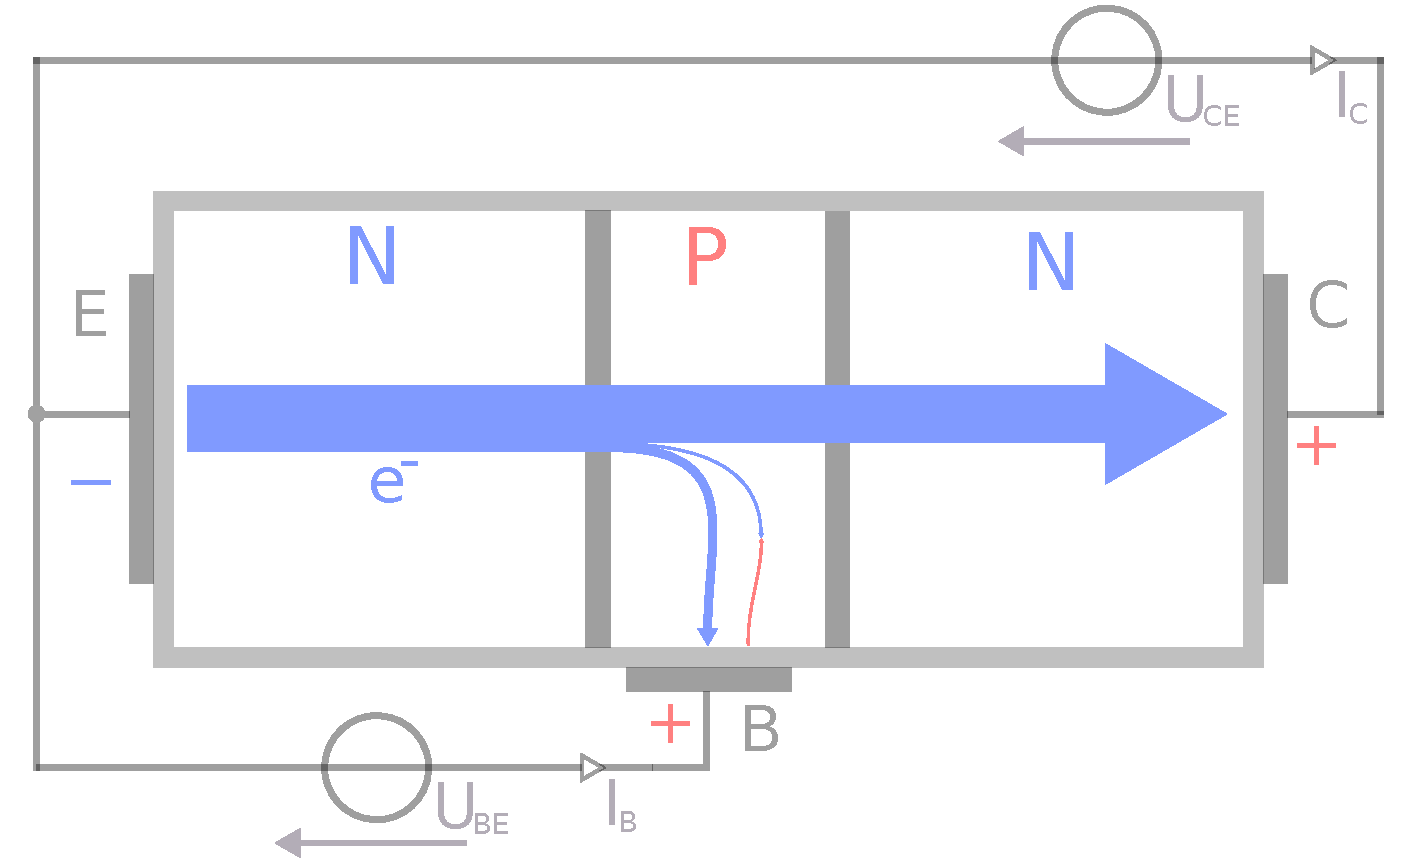
\includegraphics[width=\textwidth]{1_1/npn_voltage_both}
\end{center}

Legt man nun eine zusätzliche Spannung $U_\textrm{CE}$ an die
Kollektor-Emitter-Strecke, gelingt ein deutlich höherer Diffusionsstrom $I_\textrm{C}$ (im
Vergleich zum Basisstrom) durch den hohen Dotierungskonzentrationsunterschied
zwischen Emitter und Kollektor; Die Elektronen des Emitters diffundieren durch
die Basis in den
Kollektor. Um Rekombinationen der Emitterelektronen mit den Fehlstellen in der Basis
zu vermeiden, sollte die Basis eine geringe Weite besitzen.

\subsection{4-Quadranten-Kennlinienfeld}

\begin{center}
  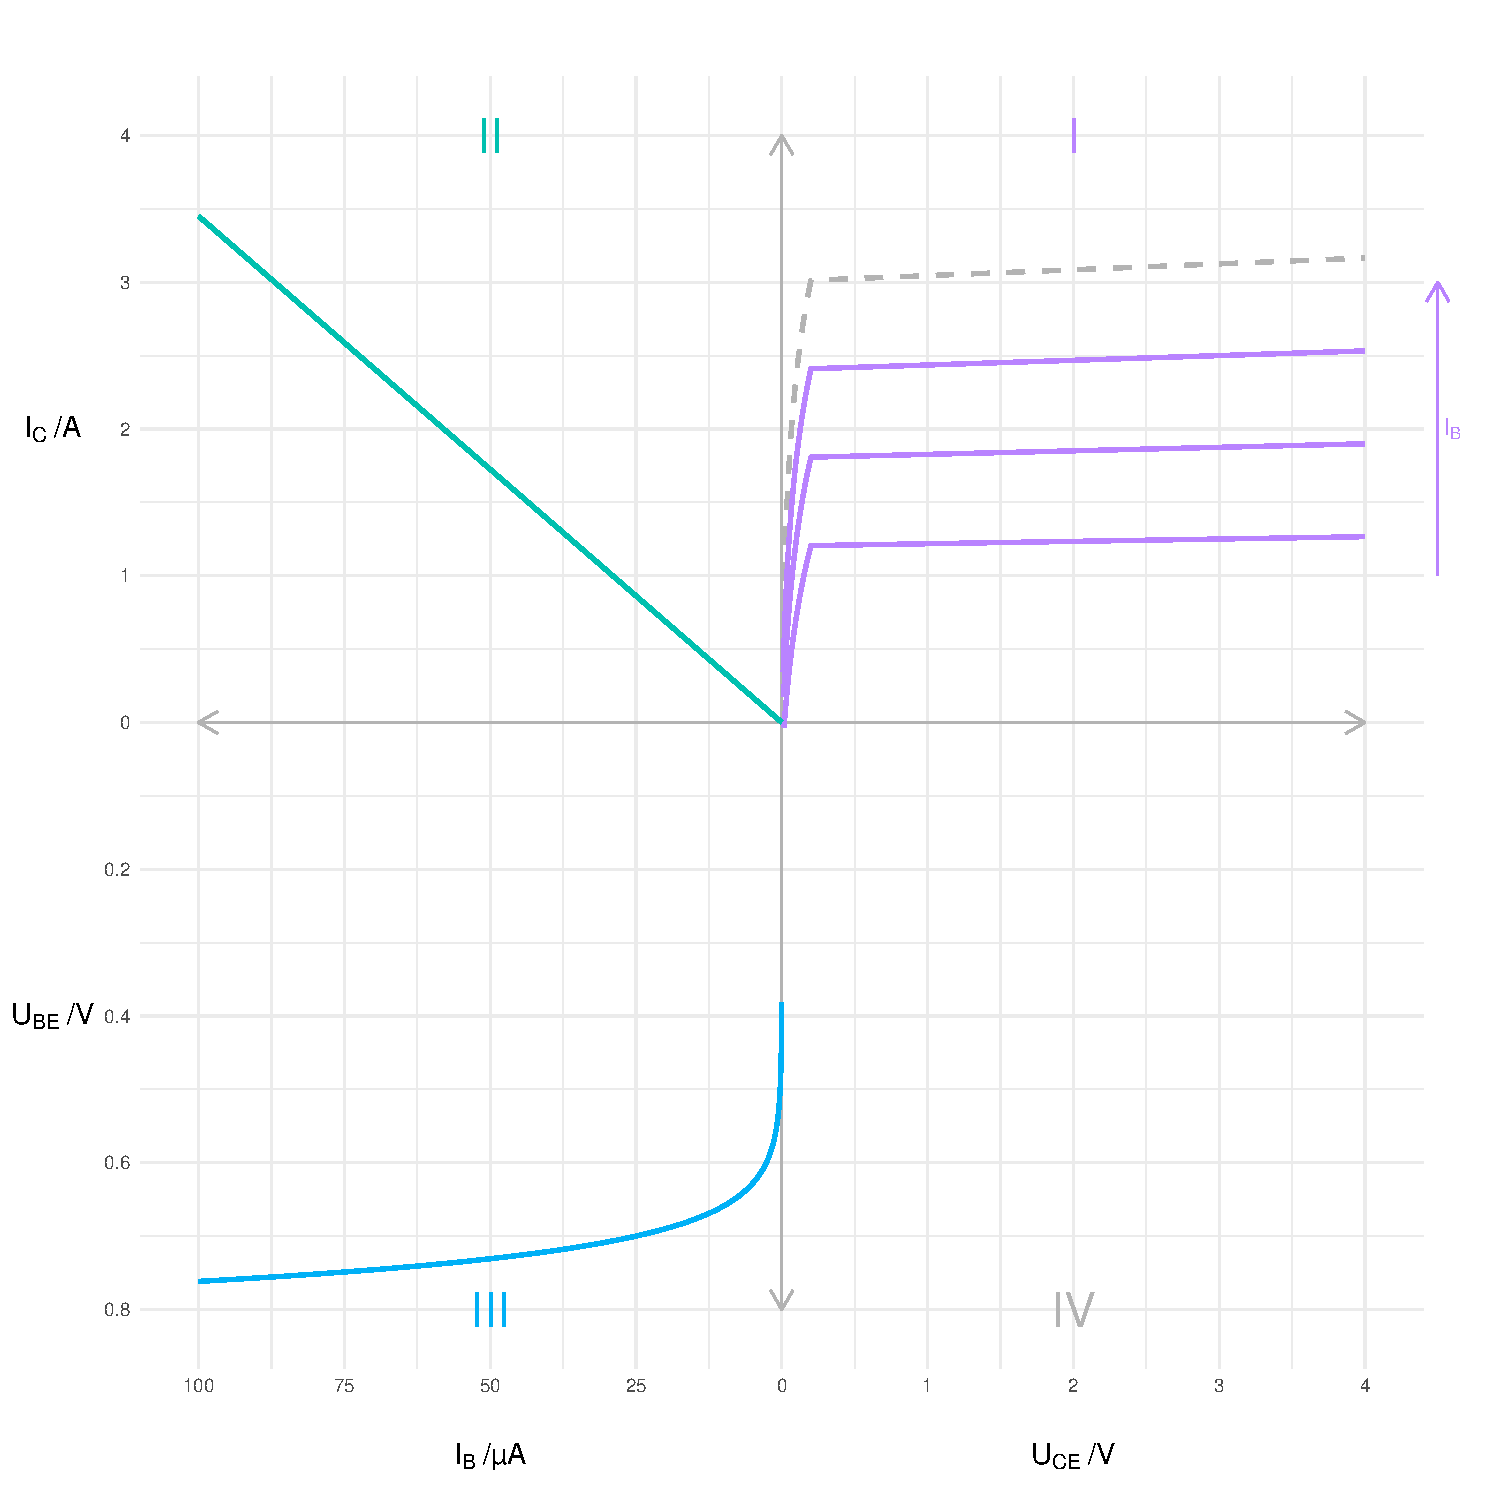
\includegraphics[width=\textwidth]{1_2/2_1_4Q}
\end{center}

Quadrant I stellt die Abhängigkeit des Kollektorstroms $I_{\textrm{C}}$ von der
Kollektor-Emitter-Spannung $U_{\textrm{CE}}$ dar. Da diese zusätzlich stark vom
Basistrom $I_{\textrm{B}}$ abhängig ist, kann keine einzelne Kennlinie
angegeben werden und es ergibt sich ein Kennlinienfeld, von dem ausgewählte
Kennlinien dargestellt werden.

Die \emph{Stromsteuerkennlinie} in Quadrant II zeigt den Zusammenhang
zwischen Eingangsstrom (Basis) und Ausgangsstrom (Kollektor). Das
Verhalten ist hier annäherungsweise linear; der statische Verstärkungsfaktor,
auch Gleichstromverstärkungsfaktor, kann daher als
$$B = \frac{I_C}{I_B}$$
ausgedrückt werden, welcher demnach nur für \textit{einen} statisch eingestellten Arbeitspunkt gilt. 

Im Quadranten III, auch \emph{Eingangskennlinienfeld}, kann durch Verfolgen der Eingangsgrößen Basis-Spannung und -Strom das
Diodenverhalten des Basis-Emitter-pn-Übergangs erkannt werden.

Quadrant IV stellt die Rückwirkung der Kollektor-Emitter-Spannung auf
die Basis-Emitter-Spannung dar, wird jedoch oft nicht verwendet, weshalb man
sich meist auf die Quadranten I, II und III beschränkt.


% 2
%%%%%%%%%%%%%%%%%%%%%%%%%%%%%%%%%%%%%
\pagebreak

\includepdf{./titlepage/titlepage2.pdf}
  \clearpage
\setcounter{page}{1}
%%%%%%%%%%%%%%%%%%%%%%%%%%%%%%%%%%%%%

\setcounter{section}{0}
\section{Versuchsaufgaben}



\end{document}
